\chapter{Code samples}

\section{Default request notifier}

The default request notifier class was taken from the Robospice source code and then modified to notify the DataProgress singleton of a request completion.

\begin{lstlisting}[language=java] 
 package com.octo.android.robospice.request.notifier;

import java.util.Set;

import roboguice.util.temp.Ln;
import android.os.Handler;
import android.os.Looper;
import android.os.SystemClock;

import com.octo.android.robospice.exception.RequestCancelledException;
import com.octo.android.robospice.persistence.exception.SpiceException;
import com.octo.android.robospice.request.CachedSpiceRequest;
import com.octo.android.robospice.request.listener.PendingRequestListener;
import com.octo.android.robospice.request.listener.RequestListener;
import com.octo.android.robospice.request.listener.RequestProgress;
import com.octo.android.robospice.request.listener.RequestProgressListener;

/**
 * Default implementation of RequestListenerNotifier. It will notify listeners
 * on the ui thread.
 * @author Andrew Clark
 */
public class DefaultRequestListenerNotifier implements RequestListenerNotifier {
    // ATTRIBUTES
    private final Handler handlerResponse;

    // CONSTRUCTOR    public DefaultRequestListenerNotifier() {
        handlerResponse = new Handler(Looper.getMainLooper());
    }

    private void post(final Runnable r, final Object token) {
        handlerResponse.postAtTime(r, token, SystemClock.uptimeMillis());
    }

    @Override
    public <T> void notifyListenersOfRequestNotFound(final CachedSpiceRequest<T> request, final Set<RequestListener<?>> listRequestListener) {
        post(new NotFoundRunnable(listRequestListener), request.getRequestCacheKey());
    }

    @Override
    public <T> void notifyListenersOfRequestAdded(final CachedSpiceRequest<T> request, Set<RequestListener<?>> listeners) {
        // does nothing for now
    }

    @Override
    public <T> void notifyListenersOfRequestAggregated(final CachedSpiceRequest<T> request, Set<RequestListener<?>> listeners) {
        // does nothing for now
    }

    @Override
    public <T> void notifyListenersOfRequestProgress(final CachedSpiceRequest<T> request, final Set<RequestListener<?>> listeners, final RequestProgress progress) {

        post(new ProgressRunnable(listeners, progress), request.getRequestCacheKey());
    }

    @Override
    public <T> void notifyListenersOfRequestSuccess(final CachedSpiceRequest<T> request, final T result, final Set<RequestListener<?>> listeners) {

        post(new ResultRunnable<T>(listeners, result), request.getRequestCacheKey());
    }

    @Override
    public <T> void notifyListenersOfRequestFailure(final CachedSpiceRequest<T> request, final SpiceException e, final Set<RequestListener<?>> listeners) {

        post(new ResultRunnable<T>(listeners, e), request.getRequestCacheKey());
    }

    @Override
    public <T> void notifyListenersOfRequestCancellation(final CachedSpiceRequest<T> request, final Set<RequestListener<?>> listeners) {

        post(new ResultRunnable<T>(listeners, new RequestCancelledException("Request has been cancelled explicitely.")), request.getRequestCacheKey());
    }

    @Override
    public <T> void clearNotificationsForRequest(final CachedSpiceRequest<T> request, final Set<RequestListener<?>> listeners) {

        handlerResponse.removeCallbacksAndMessages(request.getRequestCacheKey());
    }
    // INNER CLASSES
    private static class NotFoundRunnable implements Runnable {
        private final Set<RequestListener<?>> listeners;

        public NotFoundRunnable(final Set<RequestListener<?>> listeners) {
            this.listeners = listeners;
        }

        @Override
        public void run() {

            if (listeners == null) {
                return;
            }

            Ln.v("Notifying " + listeners.size() + " listeners of request not found");
            synchronized (listeners) {
                for (final RequestListener<?> listener : listeners) {
                    if (listener != null && listener instanceof PendingRequestListener) {
                        Ln.v("Notifying %s", listener.getClass().getSimpleName());
                        ((PendingRequestListener<?>) listener).onRequestNotFound();
                    }
                }
            }
        }
    }
    
    private static class ProgressRunnable implements Runnable {
        private final RequestProgress progress;
        private final Set<RequestListener<?>> listeners;

        public ProgressRunnable(final Set<RequestListener<?>> listeners, final RequestProgress progress) {
            this.progress = progress;
            this.listeners = listeners;
        }

        @Override
        public void run() {

            if (listeners == null) {
                return;
            }

            Ln.v("Notifying " + listeners.size() + " listeners of progress " + progress);
            synchronized (listeners) {
                for (final RequestListener<?> listener : listeners) {
                    if (listener != null && listener instanceof RequestProgressListener) {
                        Ln.v("Notifying %s", listener.getClass().getSimpleName());
                        ((RequestProgressListener) listener).onRequestProgressUpdate(progress);
                    }
                }
            }
        }
    }

    private static class ResultRunnable<T> implements Runnable {

        private SpiceException spiceException;
        private T result;
        private final Set<RequestListener<?>> listeners;

        public ResultRunnable(final Set<RequestListener<?>> listeners, final T result) {
            this.result = result;
            this.listeners = listeners;
        }

        public ResultRunnable(final Set<RequestListener<?>> listeners, final SpiceException spiceException) {
            this.spiceException = spiceException;
            this.listeners = listeners;
        }

        @Override
        public void run() {
            if (listeners == null) {
                return;
            }

            final String resultMsg = spiceException == null ? "success" : "failure";
            Ln.v("Notifying " + listeners.size() + " listeners of request " + resultMsg);
            synchronized (listeners) {
                for (final RequestListener<?> listener : listeners) {
                    if (listener != null) {
                        @SuppressWarnings("unchecked")
                        final RequestListener<T> listenerOfT = (RequestListener<T>) listener;
                        Ln.v("Notifying %s", listener.getClass().getSimpleName());
                        if (spiceException == null) {
                            listenerOfT.onRequestSuccess(result);
                        } else {
                            listener.onRequestFailure(spiceException);
                        }
                    }
                }
            }
        }
    }
}
\end{lstlisting}

\chapter{Further documentation}

This section includes all of the documents that were created whilst executing this project. Most of these documents were required by the waterfall model \cite{waterfall}.


\includepdf[pages=-]{docs/feedback.pdf}
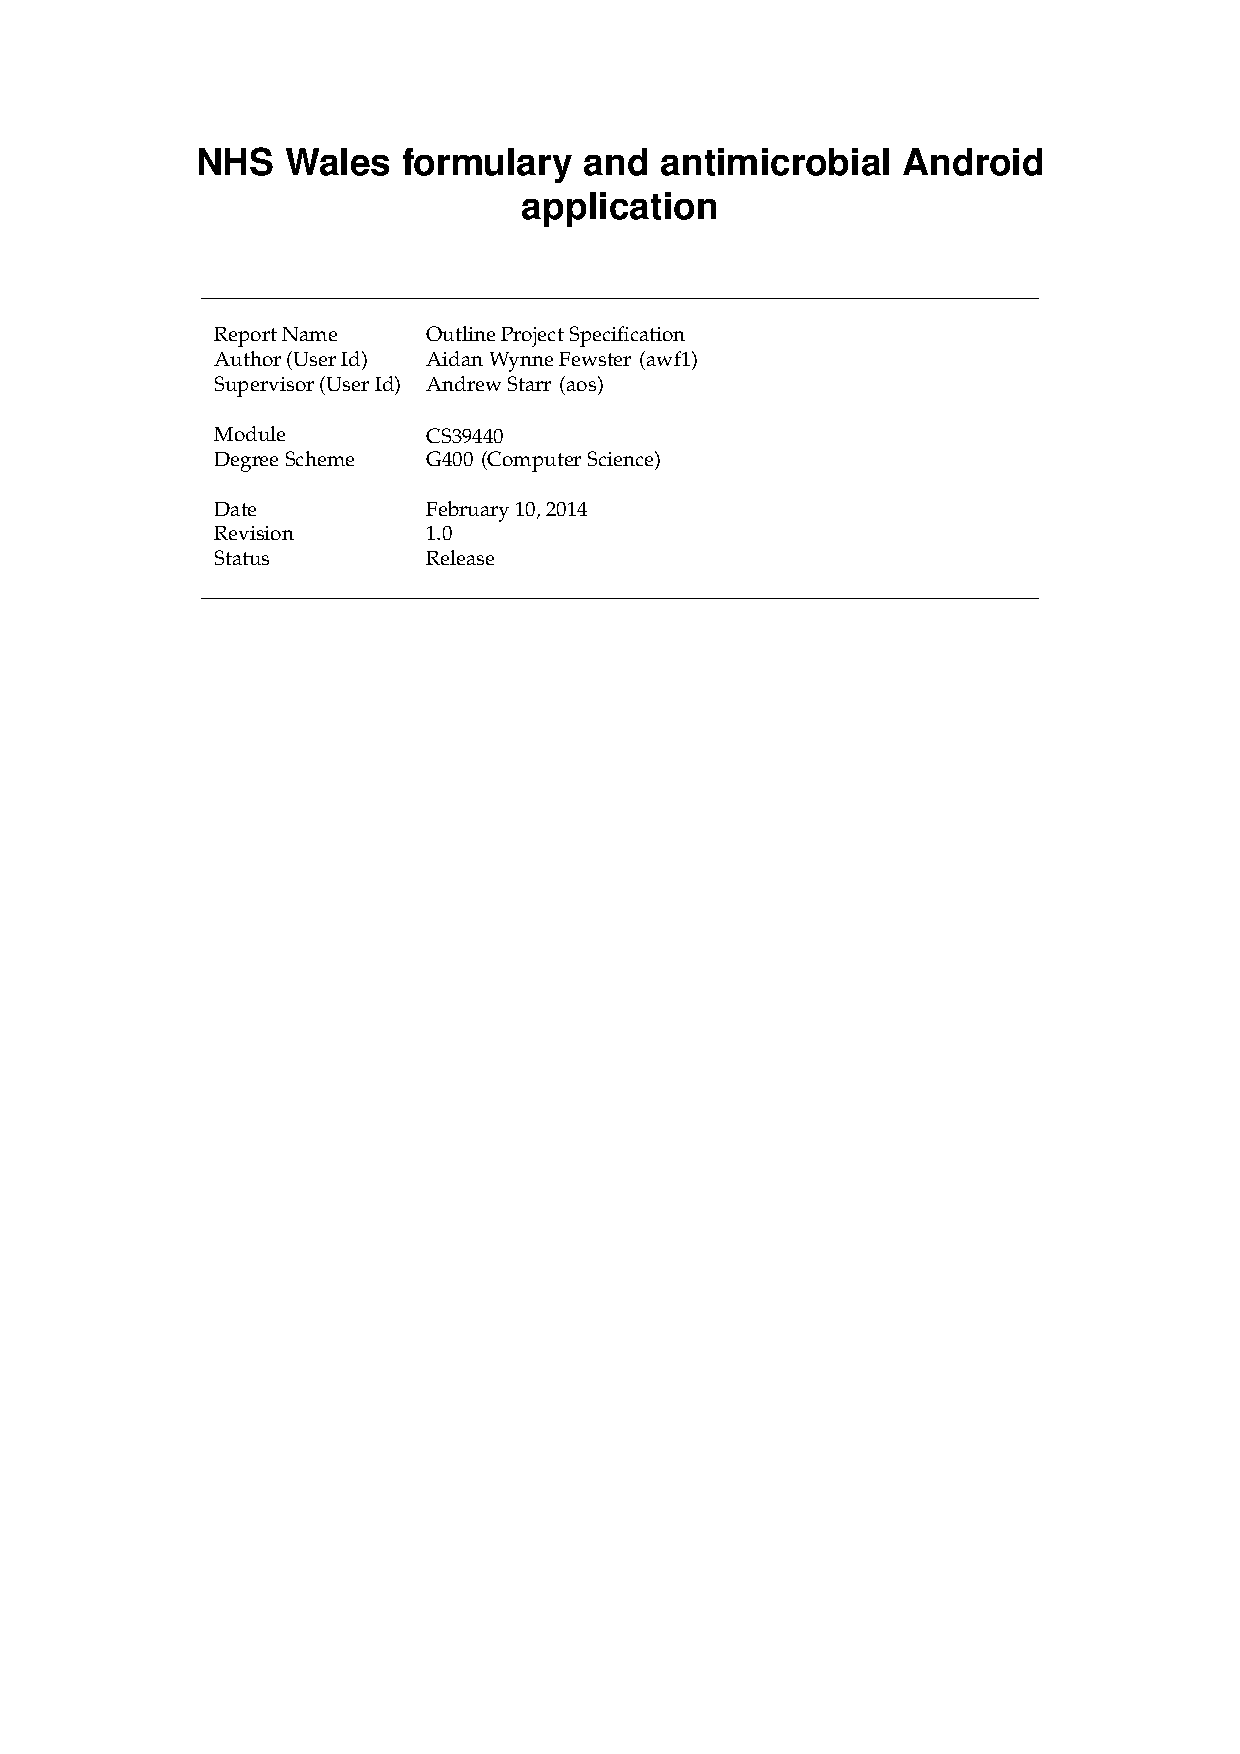
\includepdf[pages=-]{docs/outline.pdf} 
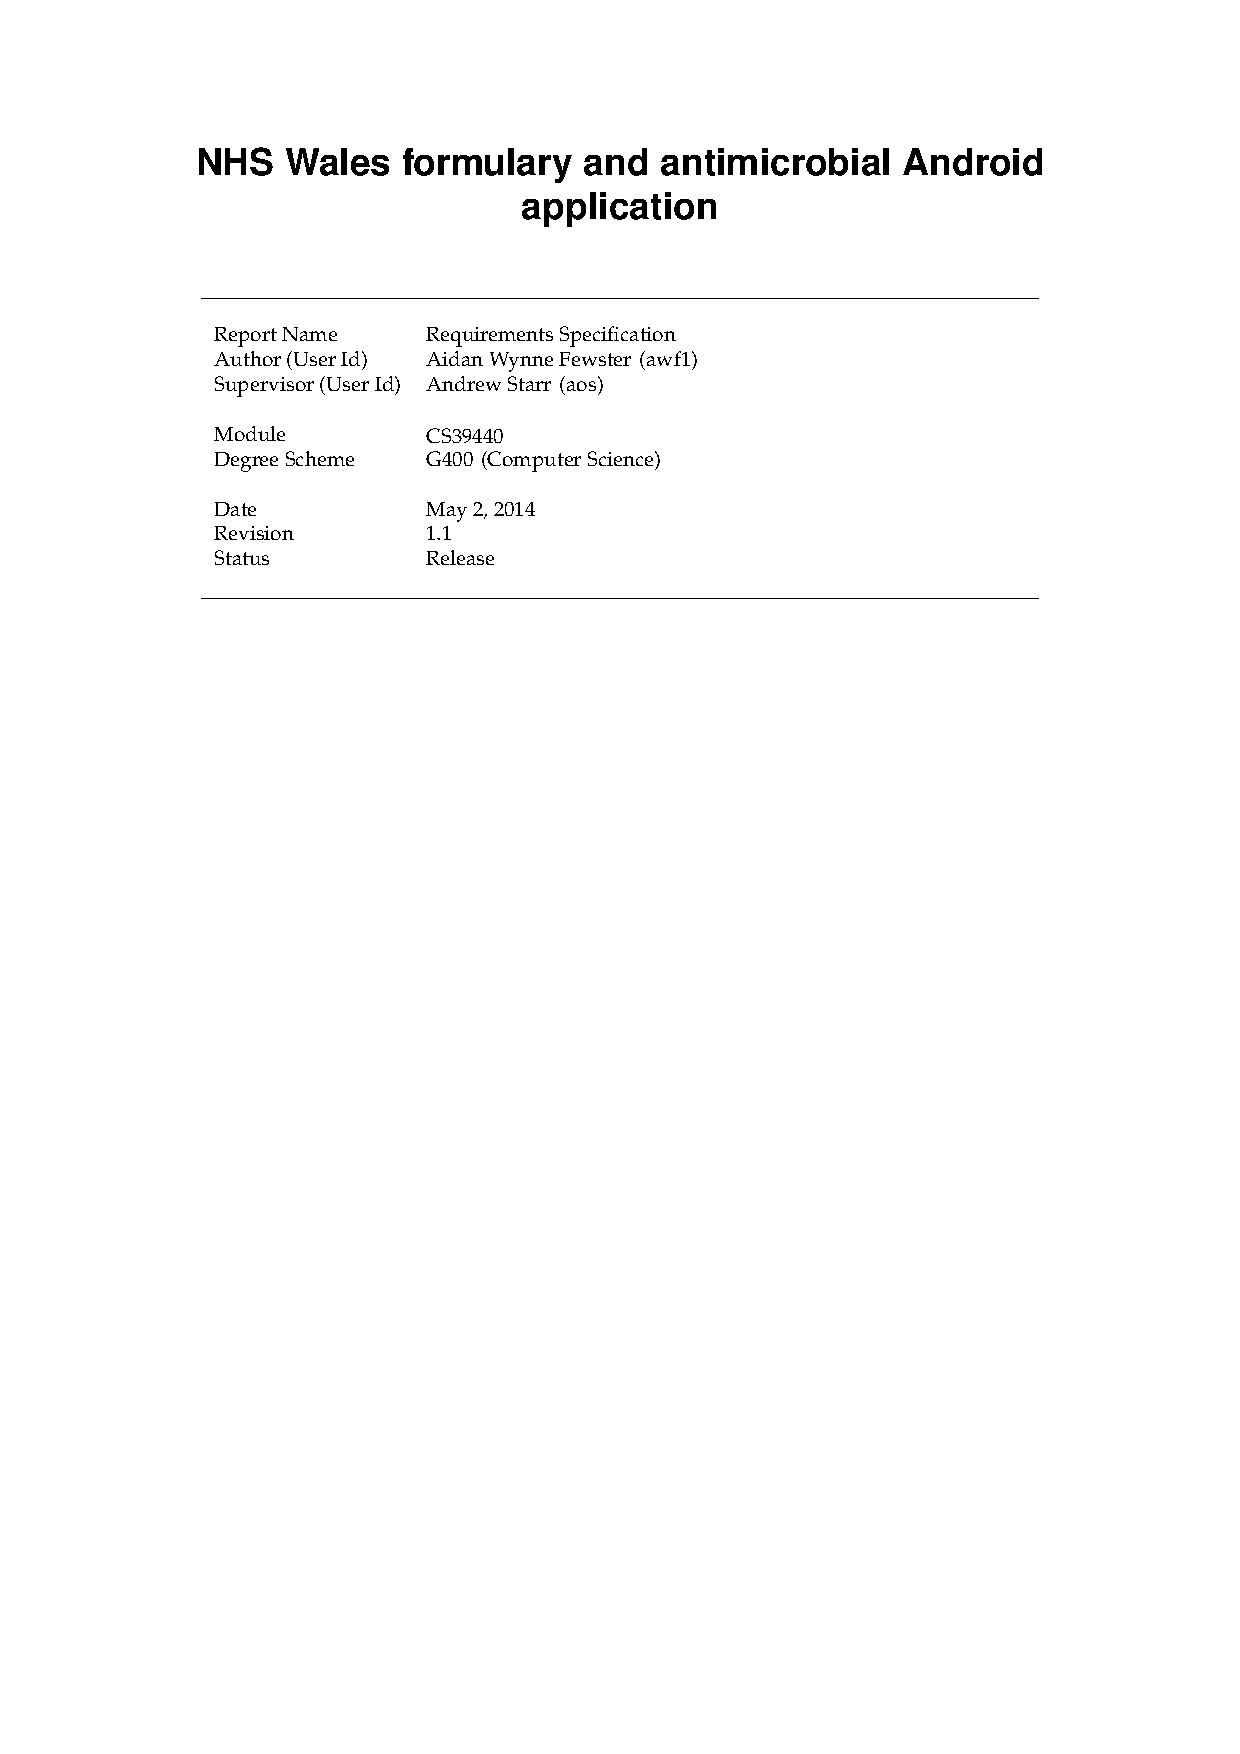
\includepdf[pages=-]{docs/req.pdf} 
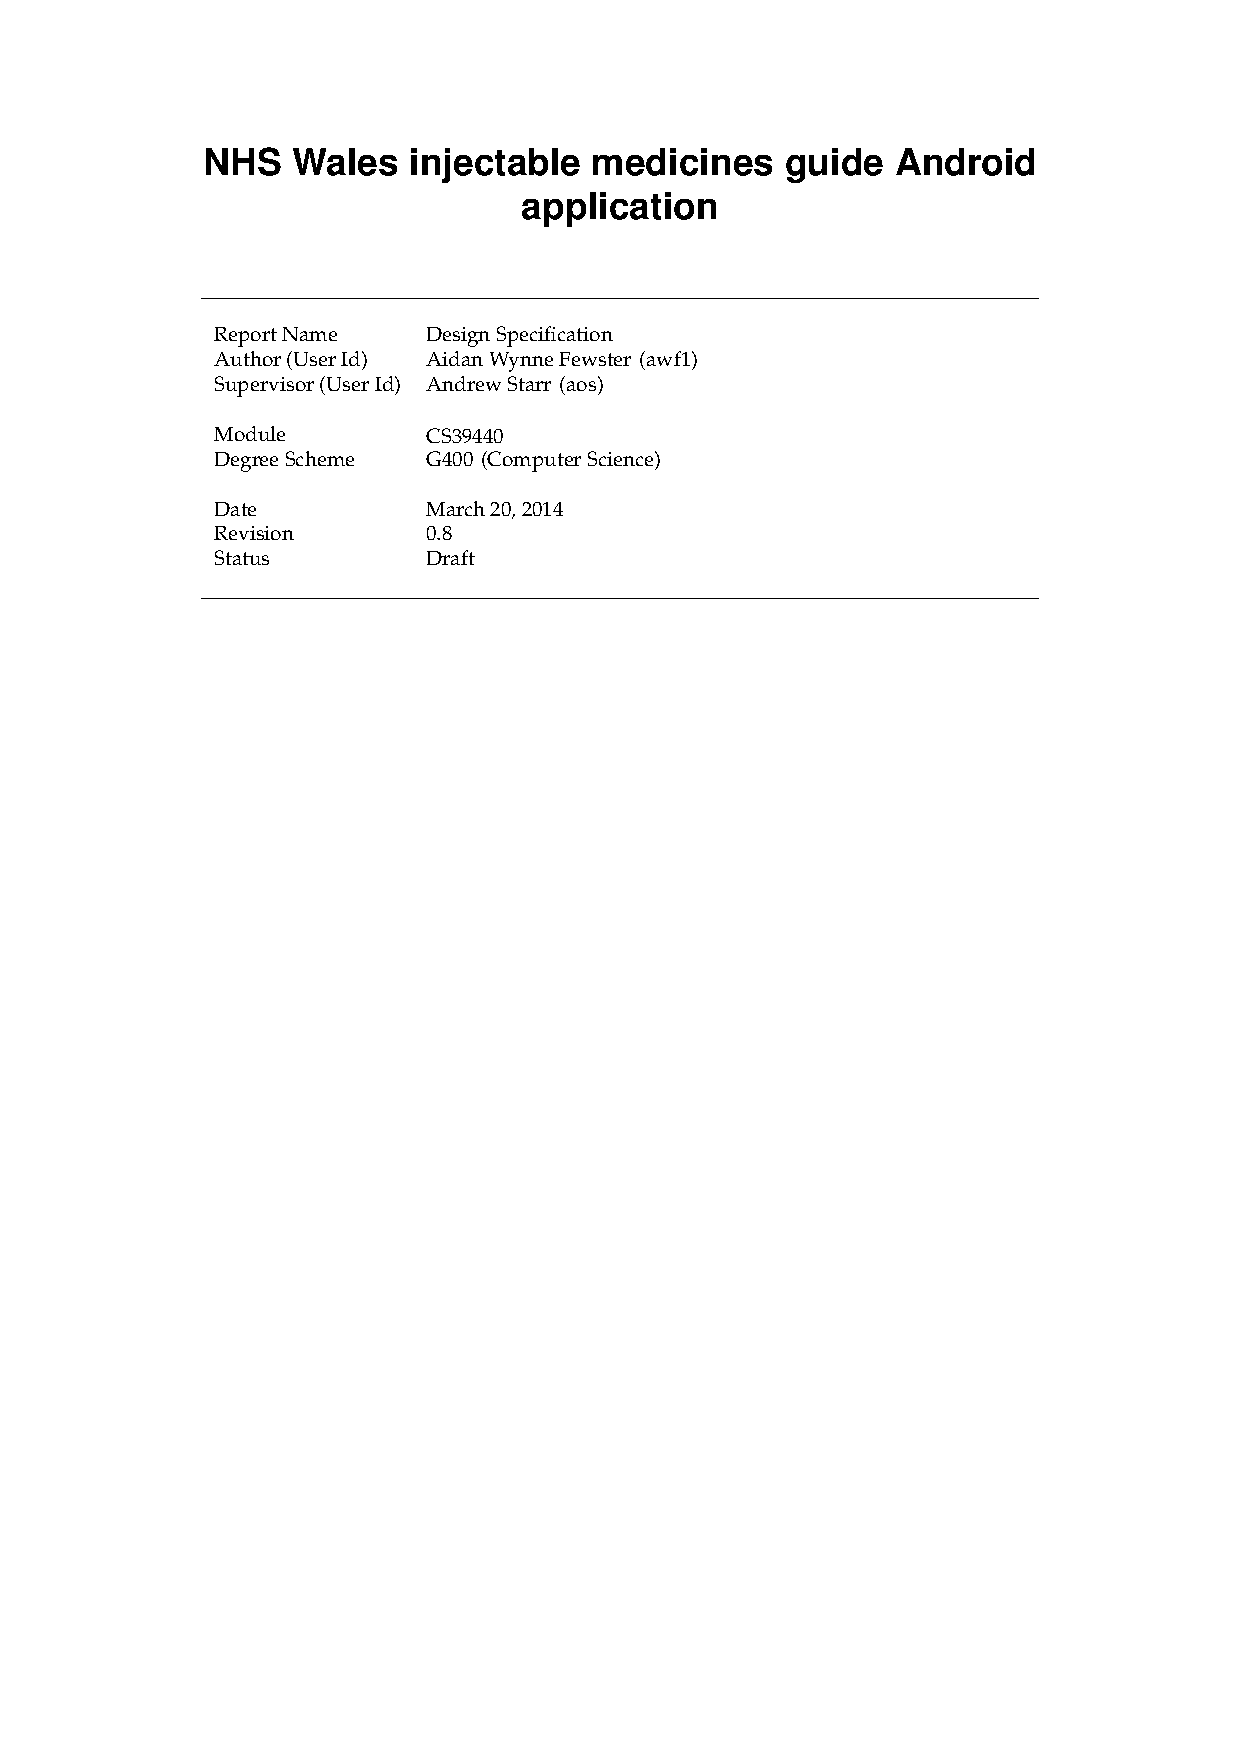
\includepdf[pages=-]{docs/design_old.pdf} 
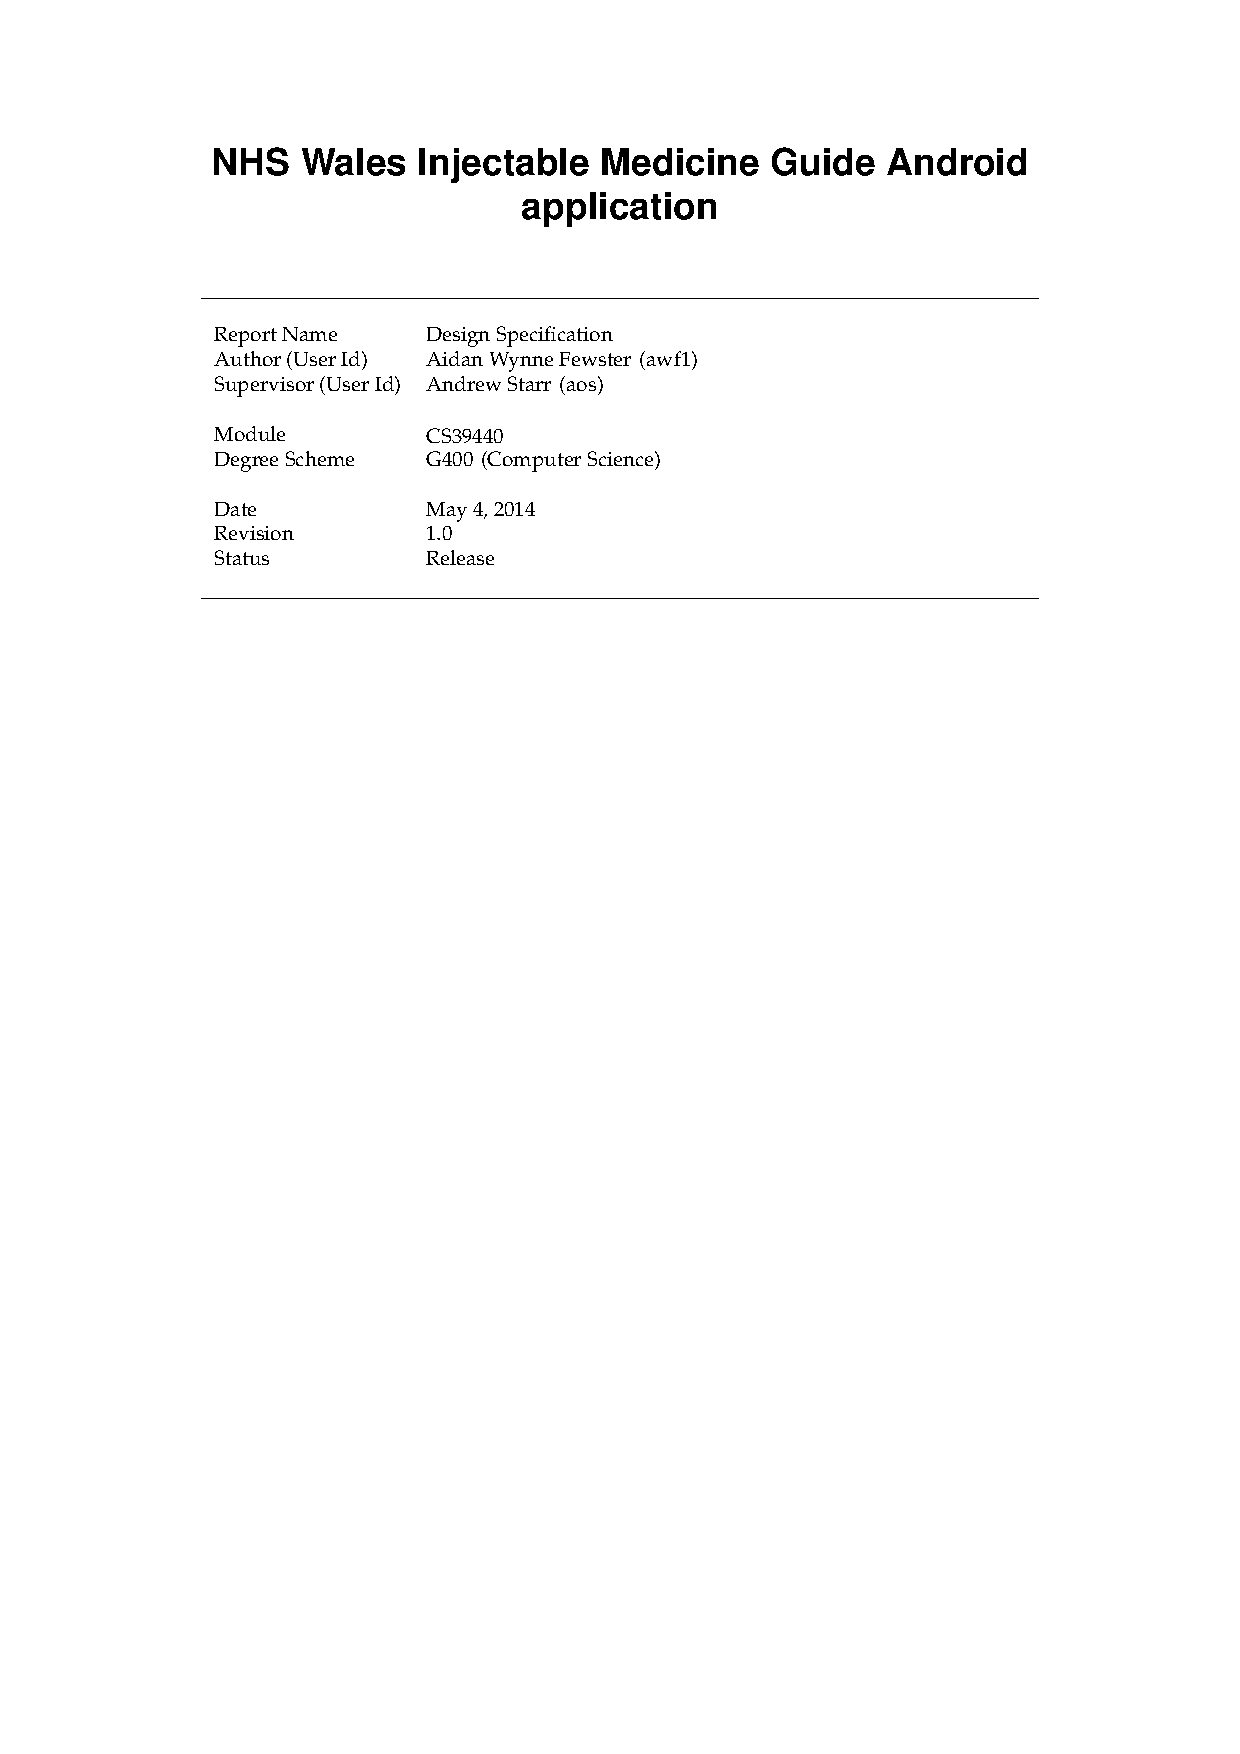
\includepdf[pages=-]{docs/design.pdf} 
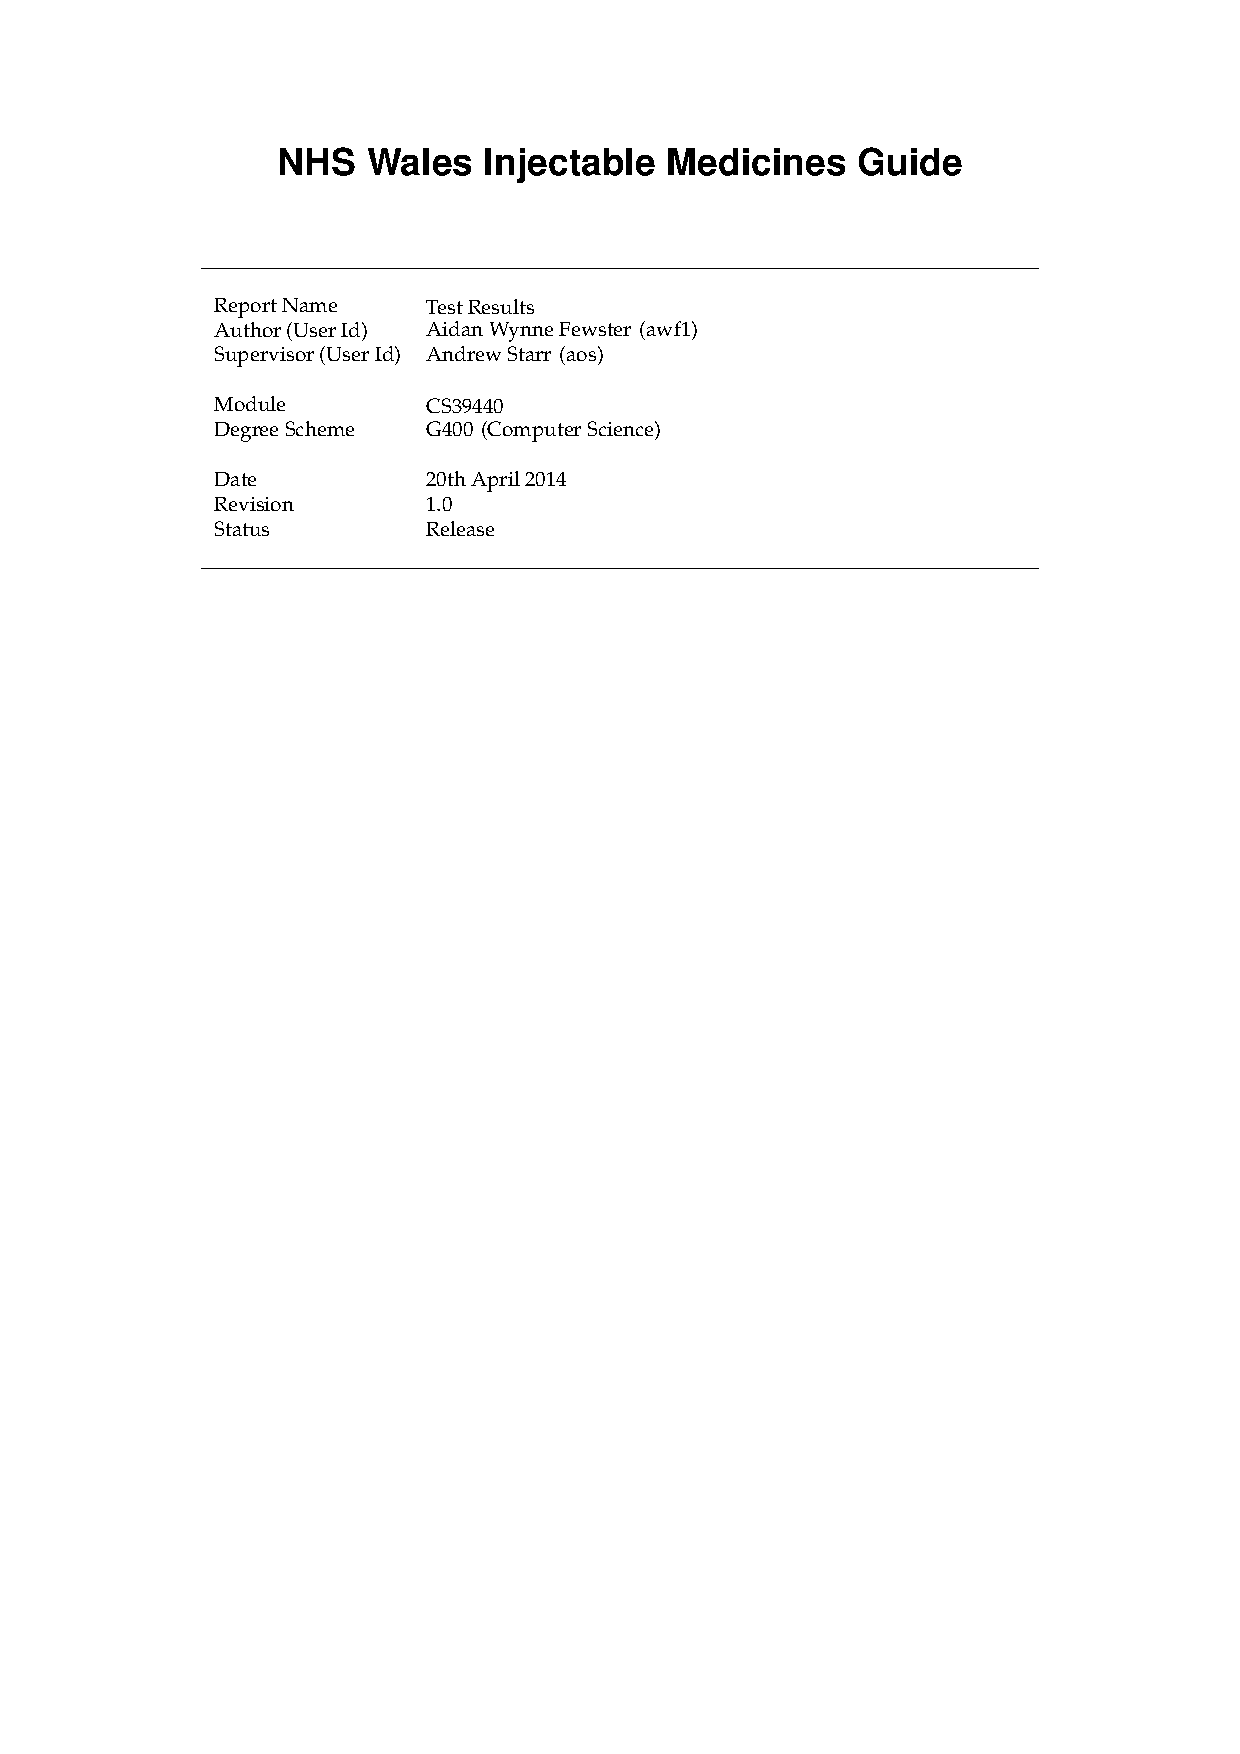
\includepdf[pages=-]{docs/test.pdf} 
